\documentclass[aspectratio=169,10pt]{beamer}

\usepackage[T1]{fontenc}
\usepackage[utf8]{inputenc}
\usepackage[spanish,es-minimal,es-noshorthands]{babel}
\usepackage{amsmath,amssymb,bm}
\usepackage{booktabs}
\usepackage{tikz}
\usetikzlibrary{positioning,arrows.meta,calc,fit,shapes.misc,decorations.pathreplacing}

\usetheme[progressbar=frametitle,numbering=fraction,sectionpage=progressbar]{metropolis}
\definecolor{azul}{HTML}{2C4A8C}
\definecolor{rojo}{HTML}{C8412C}
\definecolor{naranja}{HTML}{F4A261}
\definecolor{celeste}{HTML}{CFE6FB}
\definecolor{verde}{HTML}{2E8B57}
\definecolor{fondo}{HTML}{1F2F4A}
\setbeamercolor{frametitle}{bg=fondo,fg=white}
\setbeamercolor{progress bar}{fg=rojo,bg=celeste}
\setbeamercolor{alerted text}{fg=rojo}
\setbeamercolor{block title}{bg=celeste!70,fg=fondo}
\setbeamercolor{block body}{bg=celeste!25}
\setbeamercolor{block title alerted}{bg=rojo!85,fg=white}
\setbeamercolor{block body alerted}{bg=rojo!8}
\setbeamercolor{block title example}{bg=verde!80,fg=white}
\setbeamercolor{block body example}{bg=verde!8}
\metroset{block=fill}

\graphicspath{{imagenes/}{../figures/}}

\newcommand{\nue}{\nu_e}
\newcommand{\num}{\nu_m}
\newcommand{\figpaper}[1]{\includegraphics[width=\linewidth,height=0.80\textheight,keepaspectratio]{#1}}

\title{Plasmon-polaritones en superredes Fibonacci de metamateriales}
\subtitle{Reimplementación computacional de Reyes-Gómez \textit{et al.},
Phys.\ Rev.\ B \textbf{81}, 153101 (2010)}
\author{Emanuel Orozco Gallego}
\institute{Análisis Numérico}
\date{}

\begin{document}

\maketitle

\begin{frame}{Contenido}
  \tableofcontents[hideallsubsections]
\end{frame}

% =====================================================================
\section{El problema}
% =====================================================================

\begin{frame}{El artículo original}
  \begin{columns}[T]
    \begin{column}{0.52\textwidth}
      \textbf{Reyes-Gómez, Raigoza, Cavalcanti, de Carvalho y Oliveira}\\
      \textit{Plasmon polaritons in photonic metamaterial Fibonacci superlattices}\\
      Phys.\ Rev.\ B \textbf{81}, 153101 (2010) --- \textit{Brief Report}, 4 páginas.
      \vspace{0.6em}
      \begin{itemize}
        \item Sistema: capas de \textbf{aire} y de un \textbf{metamaterial} apiladas según la secuencia de \textbf{Fibonacci}.
        \item Luz de microondas (GHz) que incide \textbf{en oblicuo}, polarización TE.
        \item Método: \textbf{matriz de transferencia} (TMM).
        \item Resultados: 6 figuras de bandas de frecuencia.
      \end{itemize}
    \end{column}
    \begin{column}{0.44\textwidth}
      \begin{alertblock}{Pregunta física}
        Si apilamos aire y un metamaterial de índice negativo siguiendo Fibonacci
        e iluminamos en oblicuo, ¿cuántos modos \emph{luz + plasmón} aparecen y
        cómo se fragmentan al crecer la secuencia?
      \end{alertblock}
      \begin{exampleblock}{Respuesta del paper}
        Hay tantos modos como capas de metamaterial en la celda:
        \[ N_{\text{modos}} = N_B = F_{m-2}. \]
      \end{exampleblock}
    \end{column}
  \end{columns}
\end{frame}

\begin{frame}{¿Qué significa \emph{reimplementar} el paper?}
  \begin{columns}[T]
    \begin{column}{0.55\textwidth}
      \begin{enumerate}
        \item Partir \textbf{solo} de las ecuaciones y parámetros publicados.
        \item Completar lo que el paper no escribe (y documentarlo).
        \item Programar el modelo desde cero en \textbf{Python}.
        \item Verificarlo con \textbf{pruebas automáticas}.
        \item Regenerar las \textbf{6 figuras} con scripts, sin edición manual.
        \item Comparar con el original y declarar cada diferencia.
      \end{enumerate}
    \end{column}
    \begin{column}{0.41\textwidth}
      \begin{block}{Reglas del trabajo}
        \begin{itemize}
          \item Sin FDTD ni elementos finitos: solo TMM.
          \item Ningún parámetro se ajustó para ``parecerse'' al dibujo.
          \item Todo es reproducible: YAML + código + tests.
        \end{itemize}
      \end{block}
    \end{column}
  \end{columns}
\end{frame}

\begin{frame}{El sistema en una imagen}
  \centering
  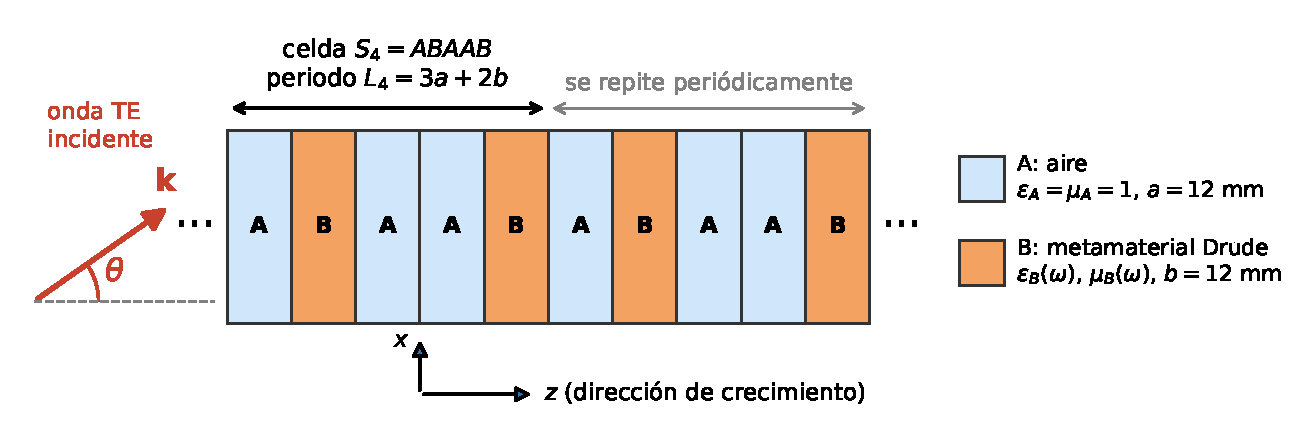
\includegraphics[width=\linewidth]{superred_geometria.pdf}
  \vspace{0.3em}
  \begin{itemize}
    \item La \textbf{celda} no es el par $AB$ sino una palabra de Fibonacci $S_m$; la celda se repite infinitamente.
    \item La onda entra con ángulo $\theta$; se estudian $\theta = 0,\ \pi/12,\ \pi/6,\ \pi/3$ ($0^\circ$, $15^\circ$, $30^\circ$, $60^\circ$).
  \end{itemize}
\end{frame}

% =====================================================================
\section{Conceptos físicos}
% =====================================================================

\begin{frame}{Ondas en materiales: $\varepsilon$ y $\mu$}
  \begin{columns}[T]
    \begin{column}{0.56\textwidth}
      Dentro de un material, la luz ``siente'' dos propiedades:
      \begin{itemize}
        \item $\varepsilon(\omega)$ --- \textbf{permitividad}: respuesta al campo eléctrico.
        \item $\mu(\omega)$ --- \textbf{permeabilidad}: respuesta al campo magnético.
      \end{itemize}
      \vspace{0.4em}
      Ambas dependen de la frecuencia. De ellas salen:
      \[
        n = \sqrt{\mu}\,\sqrt{\varepsilon}
        \qquad
        Z \propto \sqrt{\mu/\varepsilon}
      \]
      \begin{itemize}
        \item $n$: índice de refracción (velocidad de fase $c/n$).
        \item $Z$: impedancia; si dos medios tienen igual $Z$, la luz \textbf{no se refleja} en su frontera.
      \end{itemize}
    \end{column}
    \begin{column}{0.40\textwidth}
      \begin{block}{Convención de frecuencias}
        $\omega$ = frecuencia angular (rad/s)\\[0.2em]
        $\nu = \omega/2\pi$ = frecuencia en GHz\\[0.2em]
        Los ejes de todas las figuras usan $\nu$.
      \end{block}
      \begin{alertblock}{Idea clave}
        Si $\varepsilon<0$ \emph{y} $\mu<0$ a la vez, el índice es \textbf{negativo}: $n<0$.
      \end{alertblock}
    \end{column}
  \end{columns}
\end{frame}

\begin{frame}{Metamateriales: índice de refracción negativo}
  \begin{columns}[c]
    \begin{column}{0.42\textwidth}
      \centering
      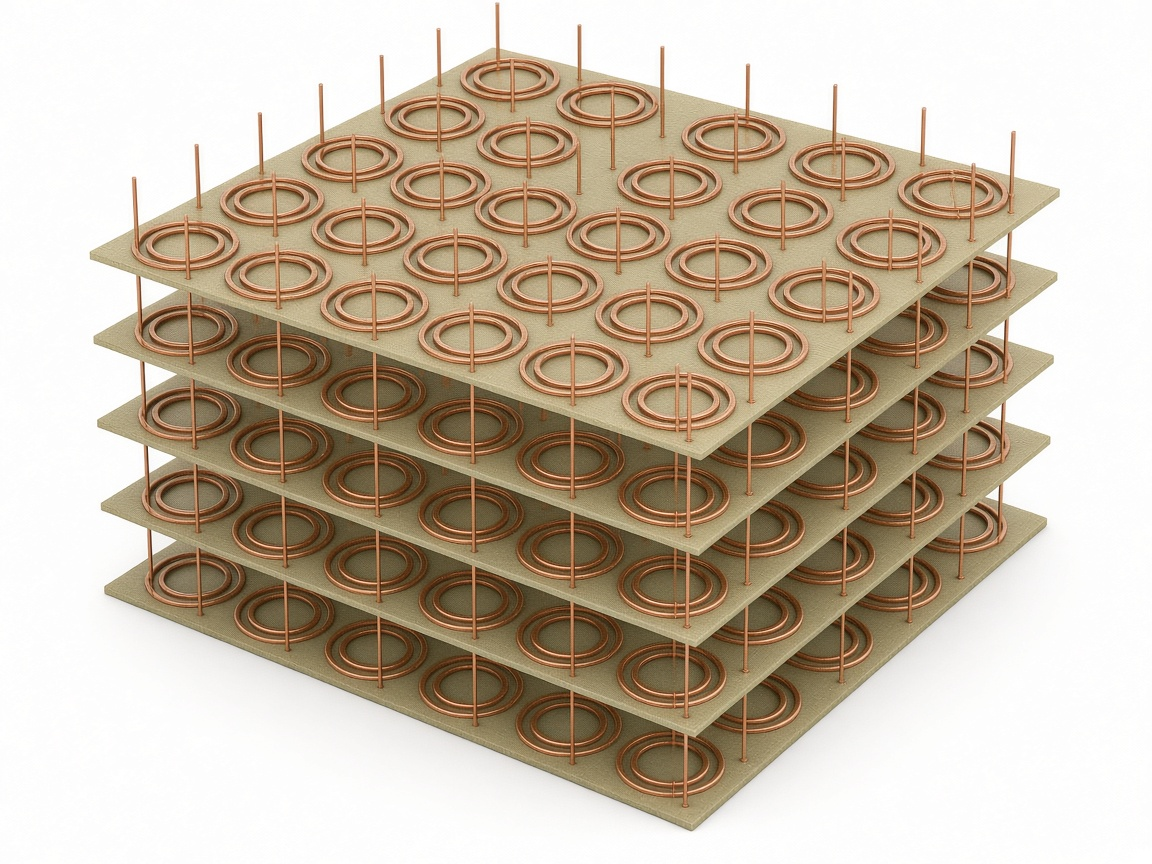
\includegraphics[width=\linewidth,height=0.72\textheight,keepaspectratio]{metamaterial_ilustracion.png}\\
      {\scriptsize Ilustración esquemática: anillos resonantes y alambres metálicos.}
    \end{column}
    \begin{column}{0.54\textwidth}
      \begin{itemize}
        \item Ningún material natural tiene $\mu<0$ en microondas.
        \item Un \textbf{metamaterial} es una estructura artificial: los \textbf{anillos} dan $\mu<0$ y los \textbf{alambres} dan $\varepsilon<0$ (Pendry, 1996).
        \item Veselago (1968): con $\varepsilon,\mu<0$ la fase viaja \emph{al revés} de la energía.
        \item El paper \textbf{no} simula los anillos: usa un modelo efectivo para toda la capa B, el \textbf{modelo de Drude}.
      \end{itemize}
    \end{column}
  \end{columns}
\end{frame}

\begin{frame}{Modelo de Drude del metamaterial (ec. 10 del paper)}
  \[
    \varepsilon_B(\omega) = 1 - \frac{\omega_e^2}{\omega^2},
    \qquad
    \mu_B(\omega) = 1 - \frac{\omega_m^2}{\omega^2}
    \qquad\text{(sin pérdidas)}
  \]
  \centering
  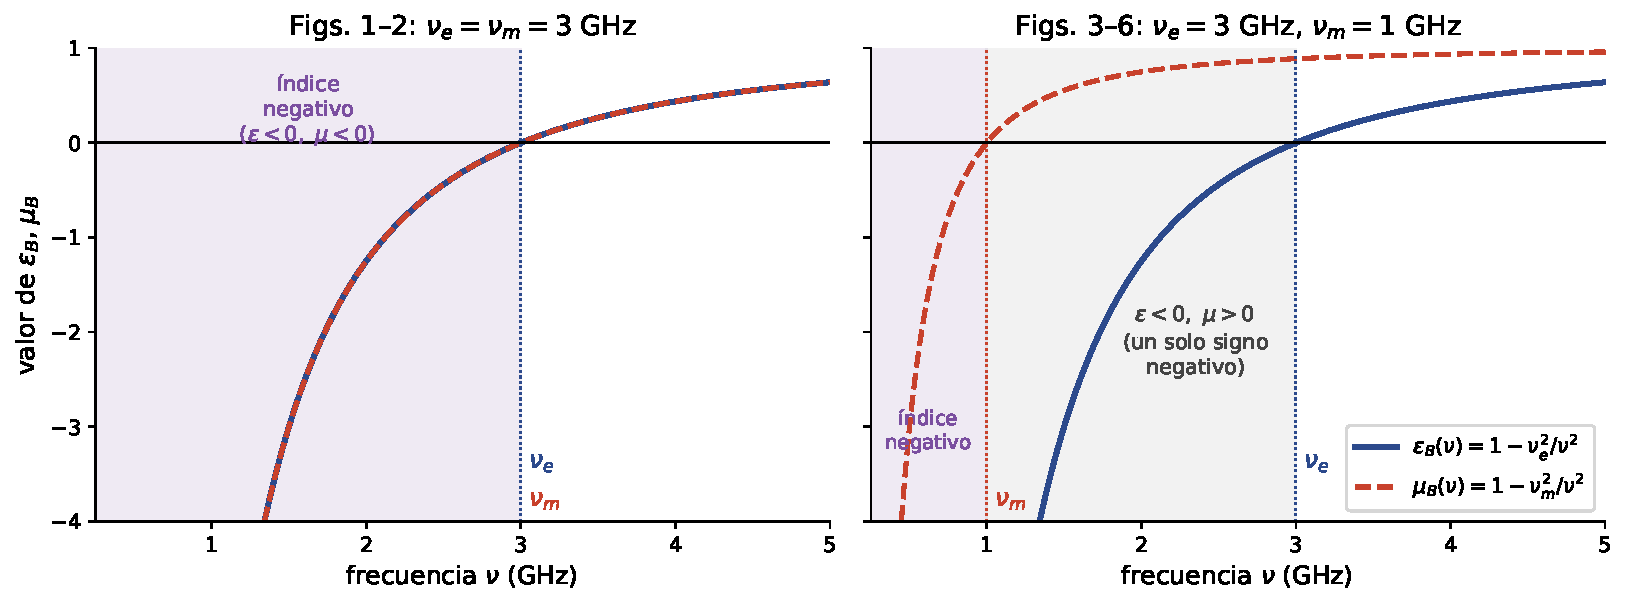
\includegraphics[width=0.92\linewidth]{drude_epsilon_mu.pdf}
  \begin{itemize}
    \item $\mu_B = 0$ en $\nu = \num$: frecuencia del \textbf{plasmón magnético}. \quad $\varepsilon_B=0$ en $\nu=\nue$.
    \item Dos juegos de parámetros: Figs.~1--2 con $\nue=\num=3$~GHz; Figs.~3--6 con $\num=1$~GHz.
  \end{itemize}
\end{frame}

\begin{frame}{Polarización TE: por qué importa el ángulo}
  \centering
  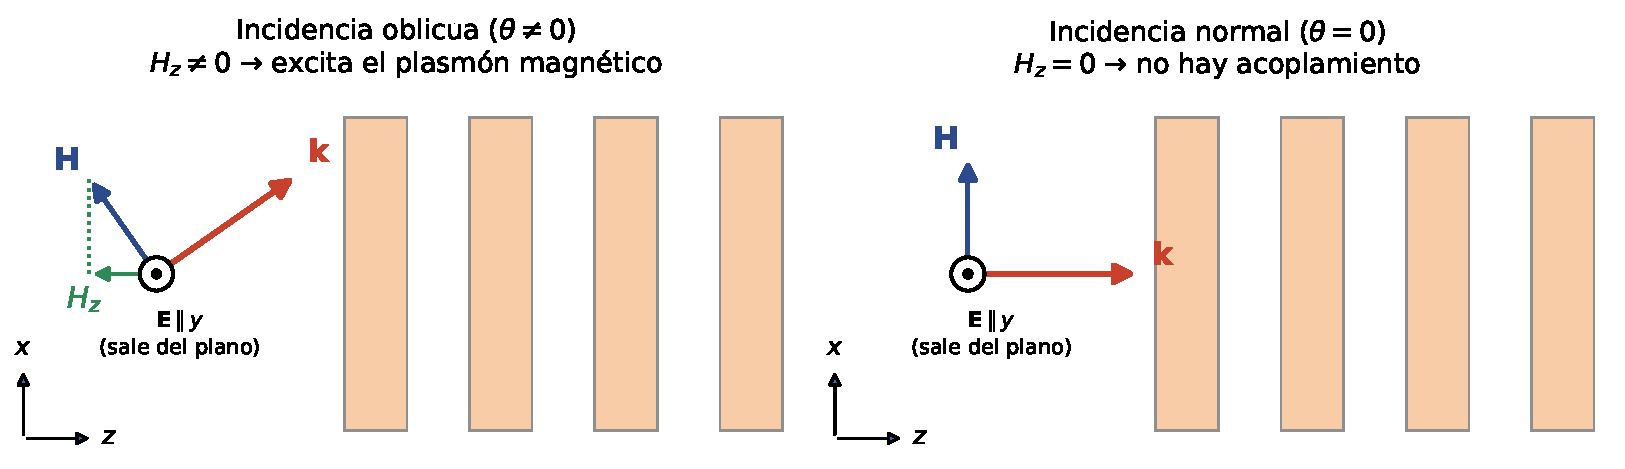
\includegraphics[width=0.95\linewidth]{polarizacion_TE.pdf}
  \begin{itemize}
    \item En TE el campo eléctrico $\mathbf{E}$ es paralelo a las capas; el magnético $\mathbf{H}$ está en el plano de incidencia.
    \item Solo la componente $H_z$ (perpendicular a las capas) puede excitar la oscilación magnética del metamaterial.
    \item A $\theta=0$ esa componente \textbf{no existe}: el acoplamiento luz--plasmón desaparece. Es geometría, no un error numérico.
  \end{itemize}
\end{frame}

\begin{frame}{Plasmones y plasmon-polaritones}
  \centering
  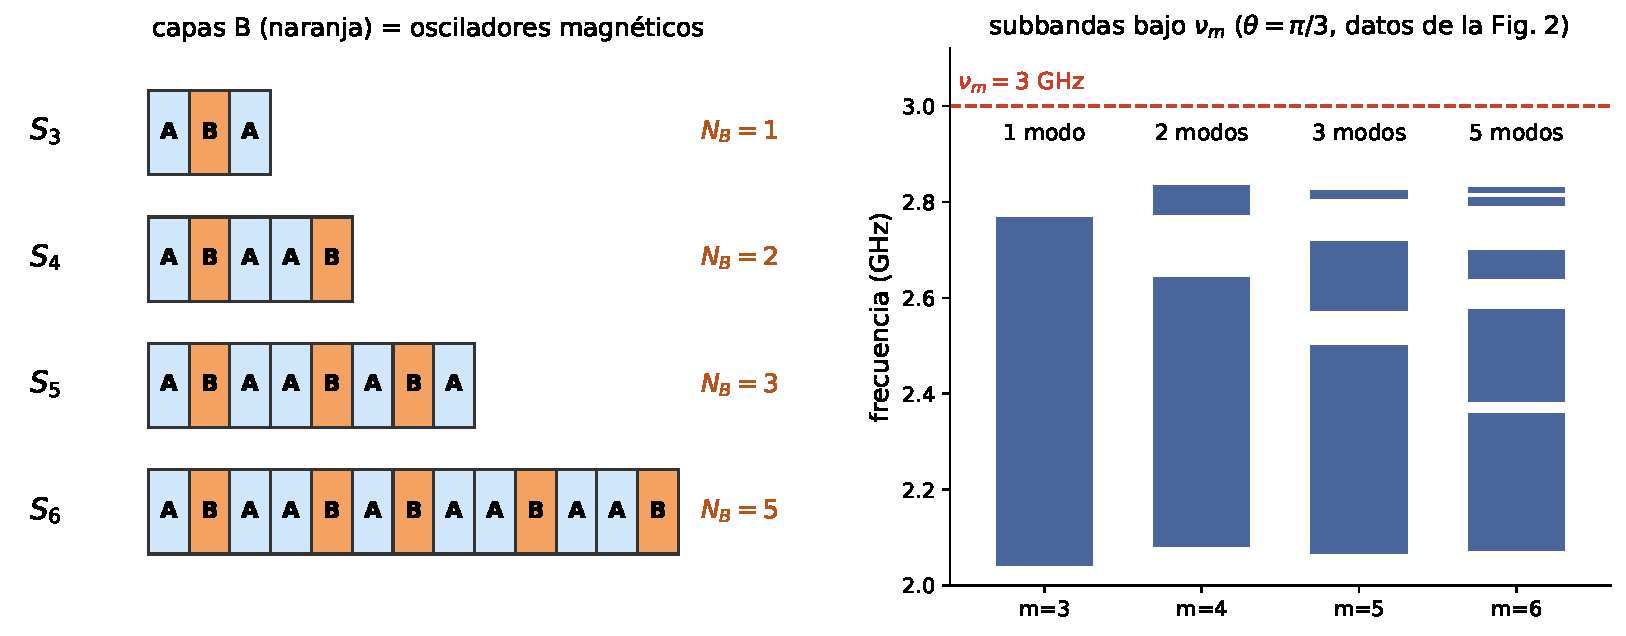
\includegraphics[width=0.93\linewidth]{osciladores_modos.pdf}
  \begin{columns}[T]
    \begin{column}{0.49\textwidth}
      \begin{itemize}
        \item \textbf{Plasmón}: oscilación colectiva del medio, aquí en $\num$ (donde $\mu_B=0$).
        \item \textbf{Polaritón}: modo híbrido \emph{luz + plasmón}.
      \end{itemize}
    \end{column}
    \begin{column}{0.49\textwidth}
      \begin{itemize}
        \item Cada capa B se comporta como un oscilador; las capas de aire los acoplan.
        \item $N_B$ osciladores acoplados $\Rightarrow$ $N_B = F_{m-2}$ modos.
      \end{itemize}
    \end{column}
  \end{columns}
\end{frame}

\begin{frame}{Cristales fotónicos: bandas y gaps}
  \begin{columns}[T]
    \begin{column}{0.37\textwidth}
      \small
      \begin{itemize}
        \item Un apilamiento periódico actúa sobre la luz como un cristal sobre los electrones.
        \item \textbf{Teorema de Bloch}: tras una celda el campo solo gana una fase
          \[ \Psi(z+L_m) = e^{ikL_m}\,\Psi(z). \]
        \item $k$ vive en $-\pi/L_m \le k \le \pi/L_m$; las figuras usan $kL_m/\pi\in[-1,1]$.
        \item \textbf{Banda}: existe $k$ real, la onda se propaga.
        \item \textbf{Gap}: no hay $k$ real, la onda decae.
      \end{itemize}
    \end{column}
    \begin{column}{0.61\textwidth}
      \centering
      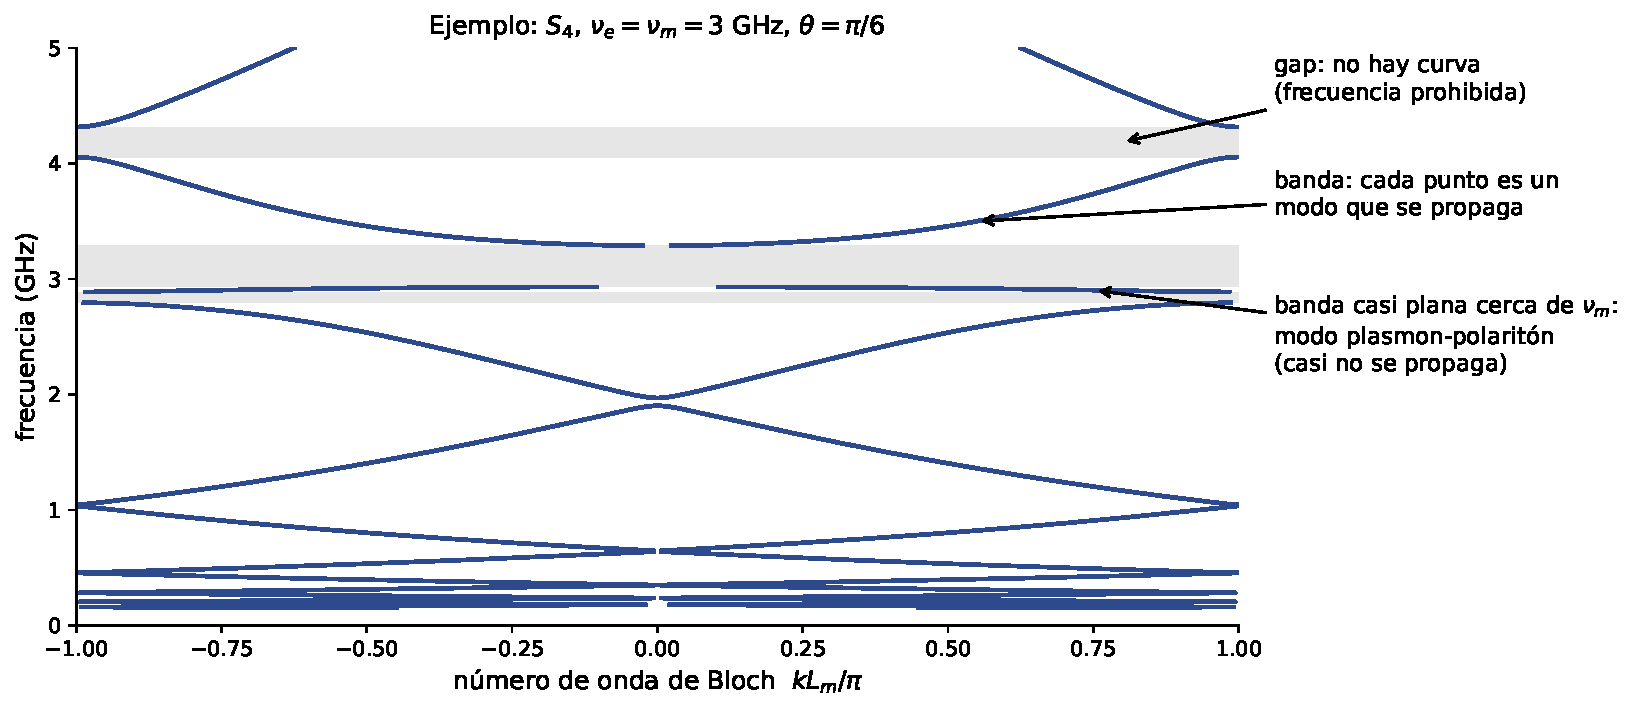
\includegraphics[width=\linewidth]{leer_dispersion.pdf}\\
      {\small Así se leen todas las figuras de resultados.}
    \end{column}
  \end{columns}
\end{frame}

\begin{frame}{El gap de índice promedio nulo $\langle n\rangle = 0$}
  \[
    \langle\varepsilon\rangle_m = \frac{F_{m-1}\,\varepsilon_A\,a + F_{m-2}\,\varepsilon_B\,b}{L_m},
    \qquad
    \langle\mu\rangle_m = \frac{F_{m-1}\,\mu_A\,a + F_{m-2}\,\mu_B\,b}{L_m}
  \]
  \centering
  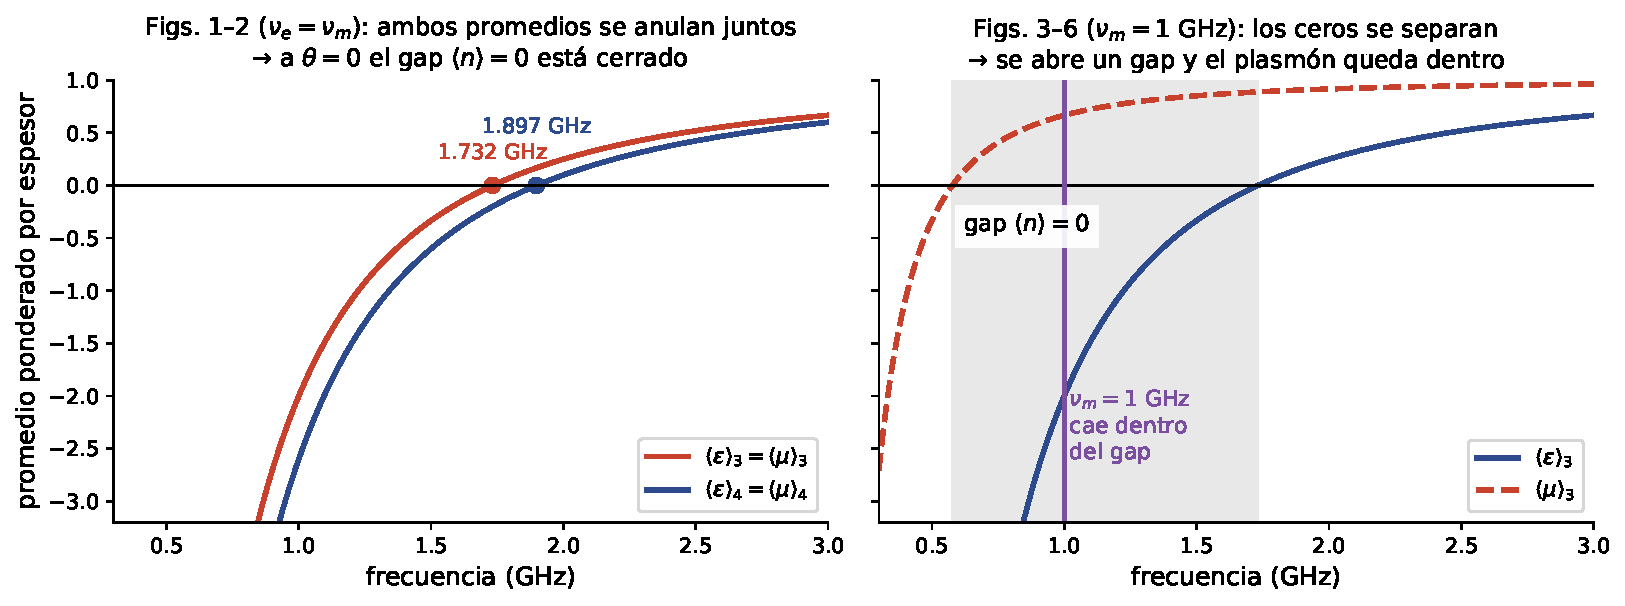
\includegraphics[width=0.92\linewidth,height=0.50\textheight,keepaspectratio]{gap_indice_nulo.pdf}
  \begin{itemize}\small
    \item Gap \textbf{no Bragg}: aparece cuando el índice promedio se anula y casi no depende del tamaño de la celda.
    \item Si $\nue=\num$ y $\theta=0$ se \textbf{cierra} en $\nu = 3\sqrt{F_{m-2}/F_m}$~GHz. Si $\num=1$~GHz, el plasmón queda \textbf{dentro} del gap.
  \end{itemize}
\end{frame}

\begin{frame}{La secuencia de Fibonacci}
  \begin{columns}[c]
    \begin{column}{0.58\textwidth}
      \centering
      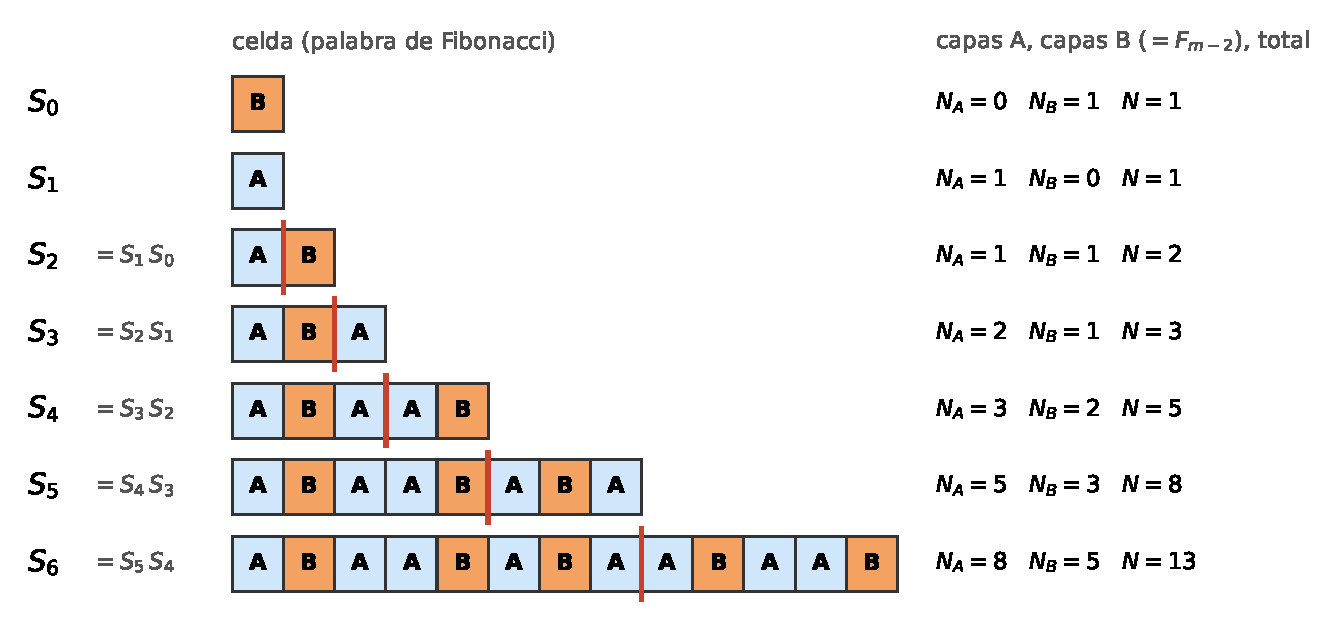
\includegraphics[width=\linewidth]{fibonacci_construccion.pdf}
    \end{column}
    \begin{column}{0.40\textwidth}
      \small
      \begin{gather*}
        S_0 = B,\quad S_1 = A,\quad S_m = S_{m-1}\,S_{m-2} \\
        F_m = F_{m-1}+F_{m-2},\quad F_0=F_1=1 \\
        L_m = F_{m-1}\,a + F_{m-2}\,b
      \end{gather*}
      \begin{itemize}
        \item La línea roja separa $S_{m-1}$ de $S_{m-2}$.
        \item Capas B en la celda: $N_B = F_{m-2}$.
        \item Con $a=b=12$~mm: $L_3 = 36$~mm, $L_6 = 156$~mm.
      \end{itemize}
    \end{column}
  \end{columns}
\end{frame}

\begin{frame}{Cuasiperiodicidad y espectro tipo Cantor}
  \begin{columns}[c]
    \begin{column}{0.50\textwidth}
      \begin{itemize}
        \item Dentro de la celda $S_m$ no hay periodo interno: el orden es \textbf{cuasiperiódico}.
        \item Al subir $m$, cada banda se \textbf{parte} en más subbandas separadas por huecos cada vez más finos.
        \item El límite es un conjunto \textbf{tipo Cantor}: autosimilar.
        \item Kohmoto, Kadanoff y Tang (1983) lo describieron para electrones; aquí aparece con luz.
      \end{itemize}
    \end{column}
    \begin{column}{0.46\textwidth}
      \centering
      \begin{tikzpicture}[x=4.8cm,y=0.62cm,line width=4pt]
        \foreach \lvl/\segs in {0/{0/1},1/{0/0.333,0.667/1},2/{0/0.111,0.222/0.333,0.667/0.778,0.889/1},3/{0/0.037,0.074/0.111,0.222/0.259,0.296/0.333,0.667/0.704,0.741/0.778,0.889/0.926,0.963/1}}{
          \foreach \a/\b in \segs { \draw[azul] (\a,-\lvl) -- (\b,-\lvl); }
          \node[left,font=\small] at (-0.02,-\lvl) {paso \lvl};
        }
        \node[font=\small,align=center] at (0.5,-4.3) {cada paso parte los intervalos:\\ así se fragmentan las bandas};
      \end{tikzpicture}
    \end{column}
  \end{columns}
\end{frame}

% =====================================================================
\section{Cómo se reimplementó}
% =====================================================================

\begin{frame}{Metodología}
  \centering
  \begin{tikzpicture}[
      caja/.style={rounded corners=4pt,draw=fondo,fill=celeste!55,line width=0.8pt,
                   minimum width=3.6cm,minimum height=1.35cm,align=center,font=\small},
      flecha/.style={-{Stealth[length=3mm]},line width=1.2pt,fondo},
      node distance=0.9cm and 1.0cm]
    \node[caja] (p) {\textbf{1. Leer el paper}\\PDF de 4 páginas};
    \node[caja,right=of p] (a) {\textbf{2. Auditoría matemática}\\qué dice, qué falta};
    \node[caja,right=of a] (e) {\textbf{3. Ecuaciones completas}\\Helmholtz, TMM, Bloch};
    \node[caja,below=of e] (c) {\textbf{4. Código Python}\\paquete \texttt{fibonacci\_tmm}};
    \node[caja,below=of a] (t) {\textbf{5. Tests automáticos}\\\texttt{pytest}};
    \node[caja,below=of p,fill=naranja!45] (f) {\textbf{6. Figuras y comparación}\\PNG/PDF/SVG + JSON};
    \draw[flecha] (p) -- (a);
    \draw[flecha] (a) -- (e);
    \draw[flecha] (e) -- (c);
    \draw[flecha] (c) -- (t);
    \draw[flecha] (t) -- (f);
    \draw[flecha,dashed,rojo] (f.north) to[bend left=25] node[midway,left,font=\scriptsize,align=right] {diferencias\\$\to$ se documentan} (p.south);
  \end{tikzpicture}
  \vspace{0.6em}

  {\small Resultado: biblioteca \texttt{src/fibonacci\_tmm/}, un YAML por figura en \texttt{configs/}, un script por figura en \texttt{scripts/}.}
\end{frame}

\begin{frame}{Auditoría: lo que el paper dice y lo que no}
  \begin{columns}[T]
    \begin{column}{0.40\textwidth}
      Cada afirmación del modelo se etiquetó:
      \vspace{0.3em}

      \small
      \begin{tabular}{@{}ll@{}}
        \toprule
        \texttt{[PAPER]} & escrito en el artículo \\
        \texttt{[DEDUC]} & deducción directa \\
        \texttt{[REF16]} & artículo hermano (EPL 2009) \\
        \texttt{[AMB]} & ambiguo o incompleto \\
        \texttt{[IMPL]} & decisión propia \\
        \bottomrule
      \end{tabular}
    \end{column}
    \begin{column}{0.56\textwidth}
      \begin{alertblock}{Huecos del paper y cómo se resolvieron}
        \small
        \begin{itemize}
          \item Escribe $q = n_A\sin\theta$, sin unidades correctas. Se restauró
            \[ q = \tfrac{\omega}{c}\,n_A\sin\theta \]
            como en el artículo hermano del mismo grupo.
          \item No da $c$: se usa $299\,792\,458$~m/s.
          \item No escribe la matriz de una capa: se dedujo y se validó con sus ecs.~(7)--(9).
          \item El pie de la Fig.~6 está truncado: parámetros inferidos de las Figs.~3--5.
        \end{itemize}
      \end{alertblock}
    \end{column}
  \end{columns}
\end{frame}

\begin{frame}{Ecuación de onda y vector de estado}
  Para TE, la ecuación (1) del paper es una ecuación de Helmholtz con coeficientes por tramos:
  \[
    \frac{d}{dz}\!\left[\frac{1}{\mu(z)}\frac{dE}{dz}\right]
    = -\,\varepsilon(z)\left[\frac{\omega^2}{c^2}-\frac{q^2}{n^2(z)}\right]E(z)
  \]
  \begin{columns}[T]
    \begin{column}{0.48\textwidth}
      \begin{itemize}
        \item En cada frontera, $E$ y $\mu^{-1}\,dE/dz$ son \textbf{continuos}.
        \item Se agrupan en un vector de estado
          \[ \Psi(z) = \begin{pmatrix} E(z) \\ \mu^{-1}\,dE/dz \end{pmatrix}. \]
      \end{itemize}
    \end{column}
    \begin{column}{0.48\textwidth}
      \begin{itemize}
        \item Dentro de cada capa: $E = A\cos(Qz) + B\sin(Qz)$, con
          \[ Q = \sqrt{\tfrac{\omega^2}{c^2}\,n^2 - q^2}. \]
        \item Si $Q$ es imaginario, la onda es evanescente en esa capa.
      \end{itemize}
    \end{column}
  \end{columns}
\end{frame}

\begin{frame}{Método de matriz de transferencia (TMM)}
  \centering
  \begin{tikzpicture}[x=1cm,y=1cm]
    \foreach \x/\l/\c in {0/A/celeste,1.6/B/naranja,3.2/A/celeste}{
      \fill[\c] (\x,0) rectangle ++(1.6,1.6);
      \draw[fondo] (\x,0) rectangle ++(1.6,1.6);
      \node[font=\bfseries] at (\x+0.8,0.8) {\l};
    }
    \node[below,font=\small] at (0.8,0) {$M_A$};
    \node[below,font=\small] at (2.4,0) {$M_B$};
    \node[below,font=\small] at (4.0,0) {$M_A$};
    \draw[-{Stealth},line width=1pt,rojo] (-1.4,0.8) -- (-0.1,0.8) node[midway,above] {$\Psi(0)$};
    \draw[-{Stealth},line width=1pt,rojo] (4.9,0.8) -- (6.4,0.8) node[midway,above] {$\Psi(L_3)$};
    \draw[decorate,decoration={brace,amplitude=6pt}] (0,1.75) -- (4.8,1.75) node[midway,above=6pt,font=\small] {celda $S_3 = ABA$};
    \node[right,align=left,font=\small] at (7.0,0.8) {$\Psi(L_3) = \underbrace{M_A\,M_B\,M_A}_{T_3}\,\Psi(0)$};
  \end{tikzpicture}
  \vspace{0.4em}
  \begin{columns}[T]
    \begin{column}{0.50\textwidth}
      \textbf{Una capa} ($\chi=\mu$ en TE):
      \[
        M = \begin{pmatrix}
          \cos Qd & \dfrac{\chi}{Q}\sin Qd \\[0.6em]
          -\dfrac{Q}{\chi}\sin Qd & \cos Qd
        \end{pmatrix},
        \quad \det M = 1
      \]
    \end{column}
    \begin{column}{0.46\textwidth}
      \textbf{Bloch} $\Rightarrow$ una sola ecuación escalar:
      \[
        \boxed{\;\cos(kL_m) = R_m = \tfrac12\,\mathrm{Tr}\,T_m\;}
      \]
      $|R_m|\le 1$: banda \qquad $|R_m|>1$: gap
    \end{column}
  \end{columns}
\end{frame}

\begin{frame}{De la semitraza a las bandas}
  \centering
  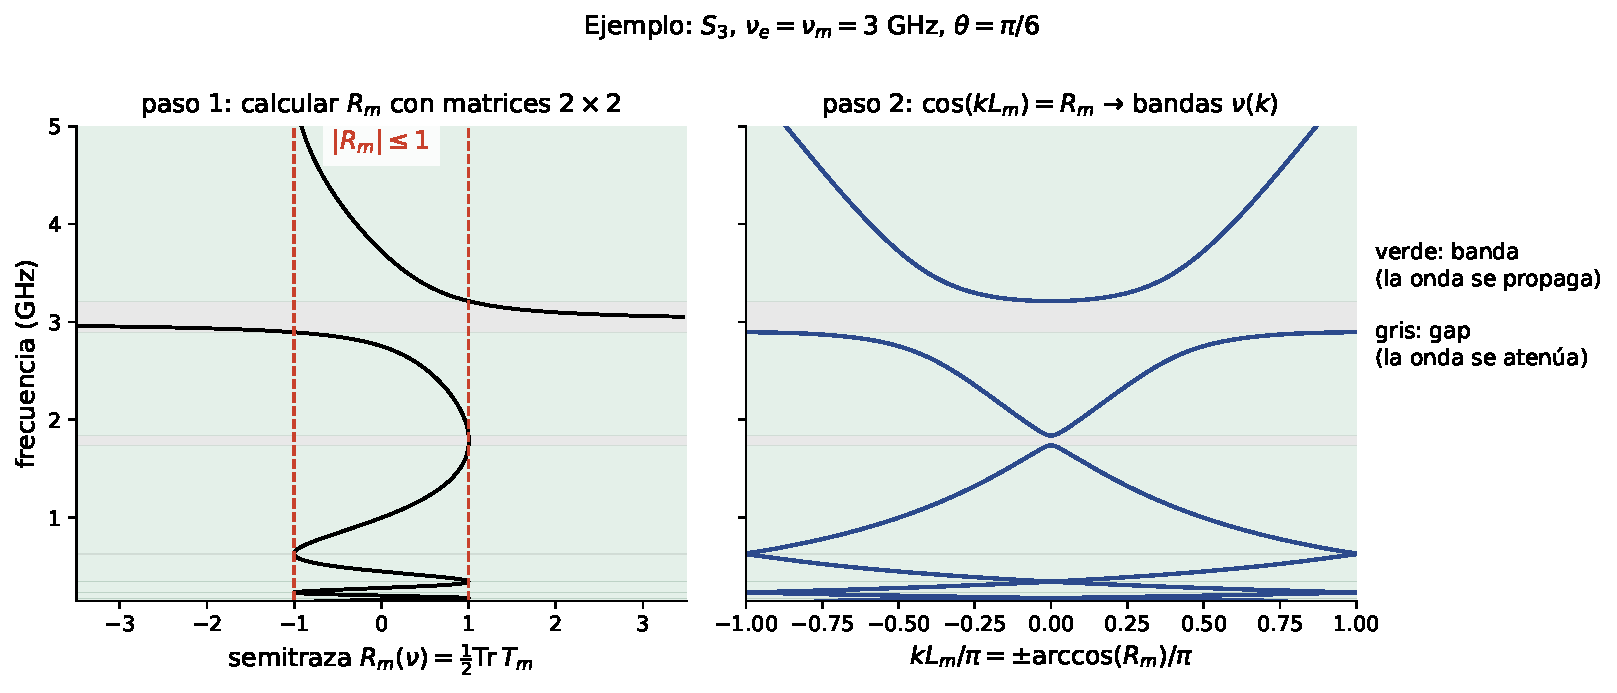
\includegraphics[width=\linewidth,height=0.72\textheight,keepaspectratio]{semitraza_bandas.pdf}
  \begin{itemize}
    \item Para cada frecuencia se calcula $R_m(\nu)$; donde $|R_m|\le 1$ se obtiene $k = \arccos(R_m)/L_m$.
    \item Barrido de 10\,000--20\,000 frecuencias por curva: cada figura tarda segundos.
  \end{itemize}
\end{frame}

\begin{frame}{Dos caminos independientes para $R_m$}
  \begin{columns}[T]
    \begin{column}{0.50\textwidth}
      \textbf{Camino 1: producto de matrices}
      \[ T_m = M_N \cdots M_2\,M_1 \]
      siguiendo la palabra $S_m$ capa por capa.
      \vspace{0.6em}

      \textbf{Camino 2: fórmulas del paper + mapa de Kohmoto}
      \begin{align*}
        R_0 &= \cos(Q_B b), \qquad R_1 = \cos(Q_A a) \\
        R_2 &= \cos(Q_A a)\cos(Q_B b) \\
            &\quad - \tfrac12\!\left[\tfrac{Q_A\mu_B}{Q_B\mu_A} + \tfrac{Q_B\mu_A}{Q_A\mu_B}\right]\sin(Q_A a)\sin(Q_B b) \\
        R_m &= 2R_{m-1}R_{m-2} - R_{m-3}
      \end{align*}
    \end{column}
    \begin{column}{0.46\textwidth}
      \begin{exampleblock}{Validación cruzada}
        El código calcula $R_m$ por los dos caminos y los tests exigen que coincidan.
        Así se confirma que la matriz de capa reconstruida reproduce las ecs.~(7)--(9) del paper.
      \end{exampleblock}
      \begin{block}{Ventaja numérica}
        La recurrencia cuesta lo mismo para cualquier $m$; el producto crece con el número de capas $F_m$.
      \end{block}
    \end{column}
  \end{columns}
\end{frame}

\begin{frame}{Arquitectura del software}
  \centering
  \begin{tikzpicture}[
      mod/.style={rounded corners=3pt,draw=fondo,fill=celeste!55,line width=0.7pt,
                  minimum height=0.95cm,minimum width=2.7cm,align=center,font=\scriptsize},
      io/.style={mod,fill=naranja!45},
      fl/.style={-{Stealth[length=2.5mm]},line width=1pt,fondo},
      node distance=0.55cm and 0.7cm]
    \node[io] (yaml) {\texttt{configs/*.yaml}\\parámetros};
    \node[mod,right=of yaml] (params) {\texttt{params.py}\\\texttt{SuperlatticeSpec}};
    \node[mod,right=1.0cm of params,yshift=1.15cm] (mat) {\texttt{materials.py}\\Drude $\varepsilon_B,\mu_B$};
    \node[mod,right=1.0cm of params] (fib) {\texttt{fibonacci.py}\\palabras $S_m$, $F_m$};
    \node[mod,right=1.0cm of params,yshift=-1.15cm] (em) {\texttt{electromagnetics.py}\\$q$, $Q$, $\chi$};
    \node[mod,right=of fib] (tmm) {\texttt{transfer\_matrix.py}\\$M$, $T_m$, $R_m$};
    \node[mod,below=1.6cm of tmm] (disp) {\texttt{dispersion.py}\\$|R|\le1$, $k(\nu)$};
    \node[mod,left=of disp] (modes) {\texttt{plasmon\_modes.py}\\\texttt{bandwidth.py}};
    \node[mod,left=of modes] (plot) {\texttt{plotting.py}\\estilo PRB};
    \node[io,left=of plot] (out) {\texttt{figures/figure\_0N/}\\PNG, PDF, SVG, JSON};
    \draw[fl] (yaml) -- (params);
    \draw[fl] (params.east) -- (mat.west);
    \draw[fl] (params) -- (fib);
    \draw[fl] (params.east) -- (em.west);
    \draw[fl] (mat.east) -- (tmm.west);
    \draw[fl] (fib) -- (tmm);
    \draw[fl] (em.east) -- (tmm.west);
    \draw[fl] (tmm) -- (disp);
    \draw[fl] (disp) -- (modes);
    \draw[fl] (modes) -- (plot);
    \draw[fl] (plot) -- (out);
    \node[draw=rojo,dashed,rounded corners,fit=(out)(plot)(modes)(disp),inner sep=6pt,
          label={[font=\scriptsize,rojo]below:\texttt{scripts/reproduce\_figure\_0N.py} orquesta cada figura}] {};
  \end{tikzpicture}
\end{frame}

\begin{frame}{Parámetros de cada figura}
  \centering
  \small
  \begin{tabular}{@{}clllll@{}}
    \toprule
    Fig. & $\nue$ (GHz) & $\num$ (GHz) & órdenes $m$ & ángulos $\theta$ & barrido en $\nu$ \\
    \midrule
    1 & 3 & 3 & 3, 4 & $0,\ \pi/12,\ \pi/6,\ \pi/3$ & 0.15--5 GHz, 12\,000 puntos \\
    2 & 3 & 3 & 3, 4, 5, 6 & $\pi/3$ & 2--4 GHz, 12\,000 puntos \\
    3 & 3 & 1 & 3, 4 & $0,\ \pi/12,\ \pi/6,\ \pi/3$ & 0.15--5 GHz, 10\,000 puntos \\
    4 & 3 & 1 & 3, 4 & $\pi/12,\ \pi/3$ & cerca de 1 GHz, 16\,000 puntos \\
    5 & 3 & 1 & 2 a 8 & $\pi/12,\ \pi/3$ & cerca de 1 GHz, 20\,000 puntos \\
    6 & 3 & 1 & 2 a 7 & 41 valores en $[0,\pi/3]$ & 0.90 GHz--$\nu_m$, 310\,000 puntos \\
    \bottomrule
  \end{tabular}
  \vspace{0.8em}

  En todas: $a=b=12$~mm, aire con $\varepsilon_A=\mu_A=1$, polarización TE.\\
  Fig.~6: parámetros \textbf{inferidos} (el pie de figura original está incompleto).
\end{frame}

\begin{frame}{Verificación y convergencia}
  \begin{columns}[c]
    \begin{column}{0.46\textwidth}
      \textbf{Tests automáticos} (\texttt{pytest}):
      \begin{itemize}
        \item Identidades de Fibonacci ($S_m$, $F_m$, inflación $A\to AB$, $B\to A$).
        \item $\det M = 1$ para toda capa.
        \item Producto de matrices = recurrencia de Kohmoto.
        \item $R_0, R_1, R_2$ = ecs.~(7)--(9) del paper.
        \item Número de modos $= F_{m-2}$.
      \end{itemize}
      \vspace{0.3em}
      \textbf{Convergencia}: desde 2\,000 puntos el ancho de banda varía menos de 0.2\,\%.
    \end{column}
    \begin{column}{0.52\textwidth}
      \centering
      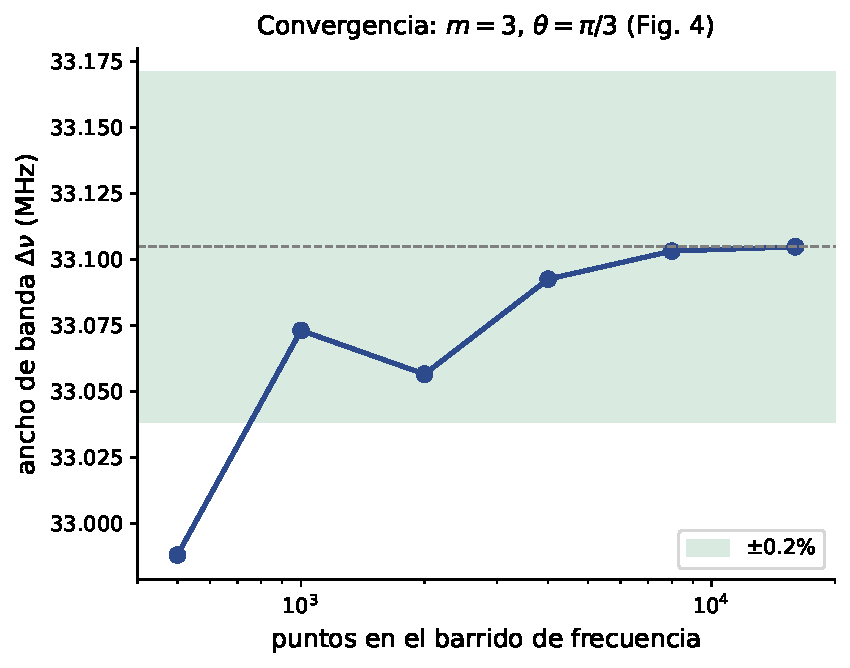
\includegraphics[width=\linewidth]{convergencia.pdf}
    \end{column}
  \end{columns}
\end{frame}

% =====================================================================
\section{Resultados}
% =====================================================================

\begin{frame}{Figura 1 --- Panorama de las bandas TE ($\nue=\num=3$ GHz)}
  \begin{columns}[c]
    \begin{column}{0.56\textwidth}
      \centering
      \figpaper{figure_01/output/figure_01.pdf}
    \end{column}
    \begin{column}{0.42\textwidth}
      \footnotesize
      \textbf{Qué se calculó:} bandas de $S_3$ (rojo discontinuo) y $S_4$ (azul) en 4 ángulos.
      \vspace{0.3em}

      \textbf{Qué se ve:}
      \begin{itemize}
        \item (a) $\theta=0$: las bandas se \textbf{cruzan} sin abrir huecos. Con $\varepsilon_B=\mu_B$ el metamaterial tiene la impedancia del aire: no hay reflexión.
        \item (b)--(d): aparece una banda \textbf{casi plana} justo debajo de $\num=3$~GHz: el plasmon-polaritón.
        \item Alrededor de esa banda se abren gaps.
      \end{itemize}
      \begin{alertblock}{Mensaje}
        \small El ángulo ``enciende'' el acoplamiento luz--plasmón.
      \end{alertblock}
    \end{column}
  \end{columns}
\end{frame}

\begin{frame}{Figura 2 --- Contar modos debajo de $\num = 3$ GHz}
  \begin{columns}[c]
    \begin{column}{0.54\textwidth}
      \centering
      \figpaper{figure_02/output/figure_02.pdf}
    \end{column}
    \begin{column}{0.44\textwidth}
      \small
      Zoom entre 2 y 4~GHz, $\theta=\pi/3$, órdenes $m=3$ a $6$. La línea roja es $\num$.
      \vspace{0.3em}

      \begin{tabular}{@{}cccl@{}}
        \toprule
        $m$ & $F_{m-2}$ & modos & intervalo total (GHz) \\
        \midrule
        3 & 1 & 1 & 2.044--2.766 \\
        4 & 2 & 2 & 2.083--2.832 (2 tramos) \\
        5 & 3 & 3 & 2.070--2.822 (3 tramos) \\
        6 & 5 & 5 & 2.075--2.827 (5 tramos) \\
        \bottomrule
      \end{tabular}
      \begin{exampleblock}{Resultado}
        \small El número de ramas es exactamente $F_{m-2}=1,2,3,5$: cada capa B añade un modo.
      \end{exampleblock}
    \end{column}
  \end{columns}
\end{frame}

\begin{frame}{Figura 3 --- El plasmón dentro del gap ($\num = 1$ GHz)}
  \begin{columns}[c]
    \begin{column}{0.56\textwidth}
      \centering
      \figpaper{figure_03/output/figure_03.pdf}
    \end{column}
    \begin{column}{0.42\textwidth}
      \small
      \textbf{Qué cambió:} ahora $\num=1$~GHz y $\nue=3$~GHz, así que $\varepsilon_B\neq\mu_B$.
      \vspace{0.3em}

      \textbf{Qué se ve:}
      \begin{itemize}
        \item (a) $\theta=0$: hueco entre $\sim$0.6 y $\sim$1.7~GHz. Es el gap $\langle n\rangle=0$, y $\num=1$~GHz cae dentro: no hay banda en 1~GHz.
        \item (b)--(d): aparece una línea \textbf{horizontal} en 1~GHz: un modo casi puramente plasmónico, que casi no se propaga.
      \end{itemize}
      \begin{alertblock}{Mensaje}
        \small Dentro del gap el polaritón queda aislado y su banda es casi plana.
      \end{alertblock}
    \end{column}
  \end{columns}
\end{frame}

\begin{frame}{Figura 4 --- Lupa sobre la banda plana de 1 GHz}
  \begin{columns}[c]
    \begin{column}{0.54\textwidth}
      \centering
      \figpaper{figure_04/output/figure_04.pdf}
    \end{column}
    \begin{column}{0.44\textwidth}
      \small
      Arriba $m=3$ (1 subbanda), abajo $m=4$ (2 subbandas). Ojo: la escala vertical cambia entre columnas.
      \vspace{0.3em}

      \begin{tabular}{@{}ccc@{}}
        \toprule
        $m$ & $\theta$ & ancho $\Delta\nu$ \\
        \midrule
        3 & $\pi/12$ & 4.5 MHz \\
        3 & $\pi/3$ & 33.1 MHz \\
        4 & $\pi/12$ & 3.5 y 0.26 MHz \\
        4 & $\pi/3$ & 26.8 y 2.5 MHz \\
        \bottomrule
      \end{tabular}
      \begin{itemize}
        \item La ``línea plana'' en realidad tiene forma de valle, con mínimo en $k=0$.
        \item El ancho crece $\sim$7 veces al pasar de $15^\circ$ a $60^\circ$: más $H_z$, más acoplamiento.
      \end{itemize}
    \end{column}
  \end{columns}
\end{frame}

\begin{frame}{Figura 5 --- Fragmentación al crecer la secuencia}
  \begin{columns}[c]
    \begin{column}{0.56\textwidth}
      \centering
      \figpaper{figure_05/output/figure_05.pdf}
    \end{column}
    \begin{column}{0.42\textwidth}
      \footnotesize
      \textbf{Cómo leerla:} cada barra vertical es un intervalo de frecuencias permitido (subbanda) cerca de 1~GHz; los colores distinguen subbandas.
      \begin{itemize}
        \item $m=2,3$: una sola barra ($F_0=F_1=1$).
        \item Desde $m=4$ cada barra se \textbf{parte}: estructura \textbf{tipo Cantor}.
        \item A $\theta=\pi/3$ el espectro ocupa unas 7 veces más rango que a $\pi/12$.
      \end{itemize}
      \begin{block}{Nota}
        \footnotesize El paper rotula el eje como ``bandwidth'', pero los valores son \emph{frecuencias}; el ancho es la longitud de cada barra.
      \end{block}
    \end{column}
  \end{columns}
\end{frame}

\begin{frame}{Conteo de modos: la regla $N = F_{m-2}$ se cumple}
  \begin{columns}[c]
    \begin{column}{0.58\textwidth}
      \centering
      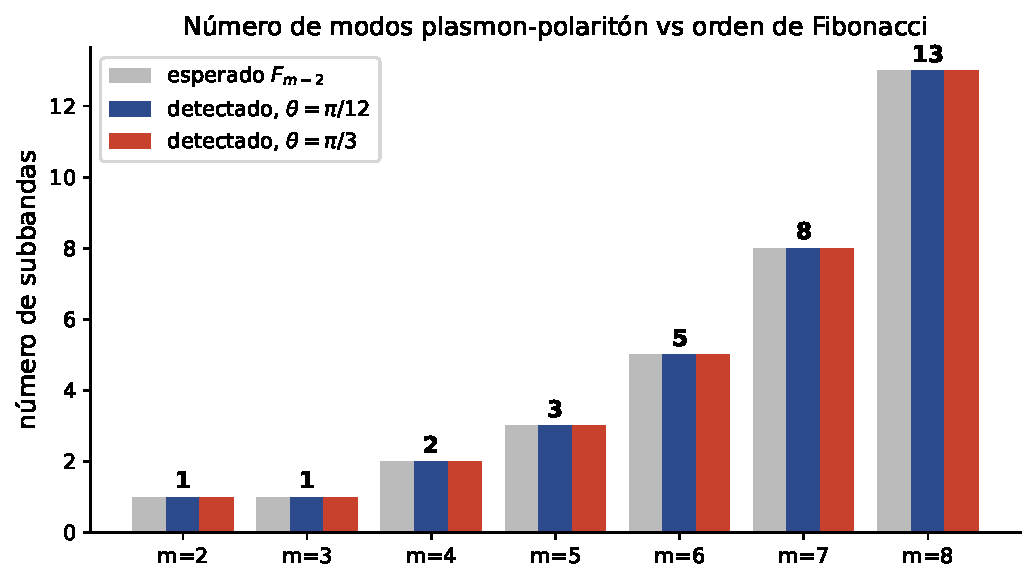
\includegraphics[width=\linewidth]{conteo_modos.pdf}
    \end{column}
    \begin{column}{0.40\textwidth}
      \small
      \begin{itemize}
        \item Conteo directo de subbandas en el cálculo: coincide \textbf{exactamente} con $F_{m-2}$ para $m=2,\dots,8$ y ambos ángulos.
        \item Hasta 13 subbandas en $m=8$, algunas de apenas $\sim$2~kHz de ancho.
      \end{itemize}
      \begin{block}{Gaps diminutos pero reales}
        \small A $\theta=\pi/12$ y $m=7$ hay gaps de solo 0.4~kHz. Son físicos ($|R_m|>1$): siguen ahí con una malla 16 veces más fina, así que no se fusionan.
      \end{block}
    \end{column}
  \end{columns}
\end{frame}

\begin{frame}{Figura 6 --- Las subbandas frente al ángulo}
  \begin{columns}[c]
    \begin{column}{0.50\textwidth}
      \centering
      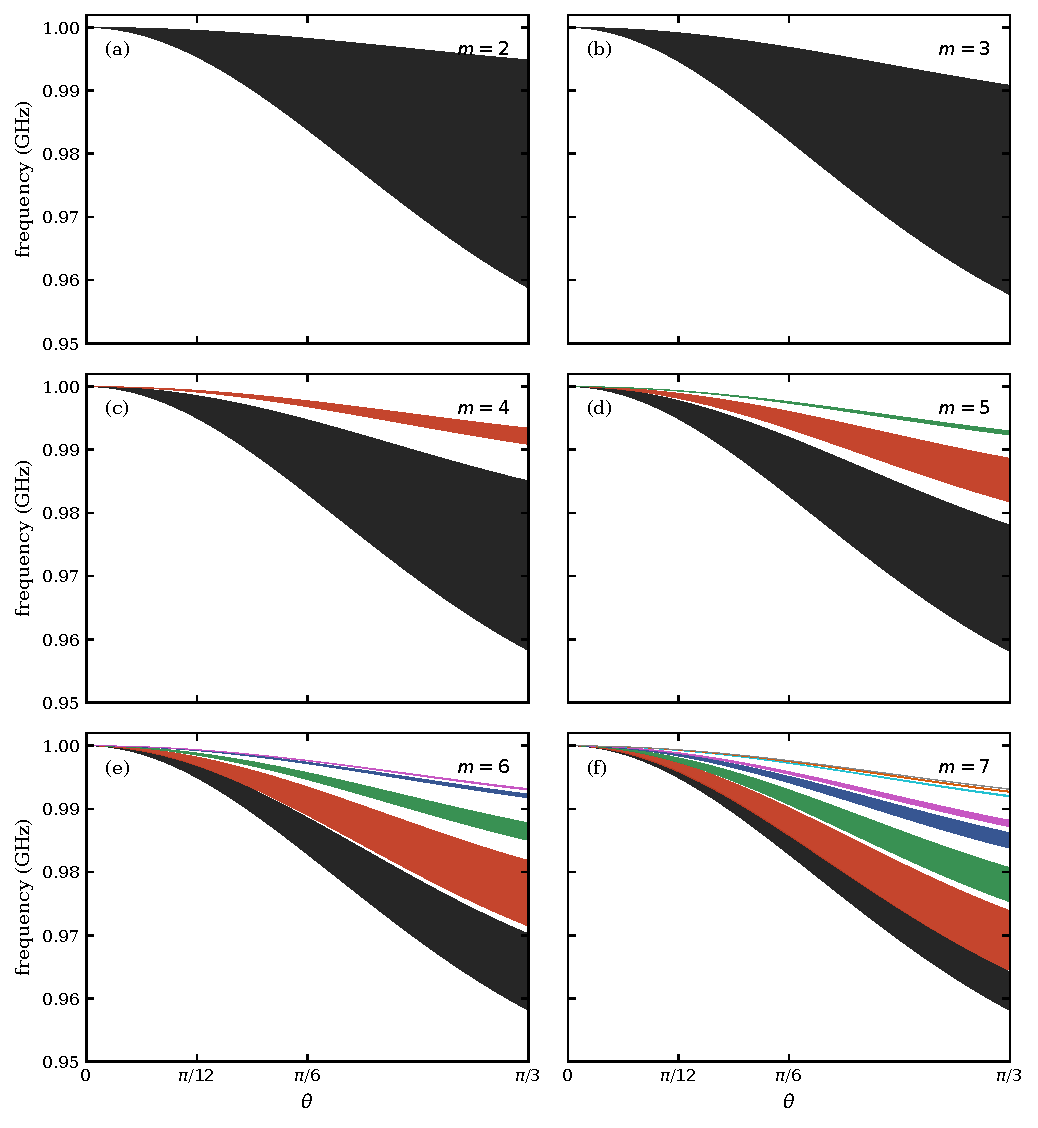
\includegraphics[width=\linewidth,height=0.84\textheight,keepaspectratio]{figure_06/output/figure_06.pdf}
    \end{column}
    \begin{column}{0.48\textwidth}
      \footnotesize
      \textbf{Cómo leerla:} eje horizontal = ángulo $\theta$; eje vertical = frecuencia. Cada región coloreada es una subbanda; su \textbf{grosor} es el ancho de banda.
      \begin{itemize}
        \item En $\theta=0$ todas colapsan en $\num=1$~GHz: sin $H_z$ no hay acoplamiento.
        \item Al crecer $\theta$ se abren hacia abajo y se ensanchan.
        \item Para todo $\theta>0$ hay exactamente $F_{m-2}$ regiones: 1, 1, 2, 3, 5, 8.
      \end{itemize}
      \begin{block}{Detalle numérico}
        \footnotesize Parámetros inferidos ($m=2..7$, $\num=1$~GHz). A ángulos pequeños las subbandas miden decenas de Hz y están pegadas a $\num$: se usa una malla logarítmica en $\num-\nu$ más una uniforme de 0.2~kHz, sin fusionar intervalos.
      \end{block}
    \end{column}
  \end{columns}
\end{frame}

\begin{frame}{Comparación con el artículo original}
  \centering
  \small
  \begin{tabular}{@{}clp{4.3cm}p{5.2cm}@{}}
    \toprule
    Fig. & Concordancia & Diferencia principal & Causa \\
    \midrule
    1 & Buena & Ninguna relevante & Mismas bandas; a $\theta=0$ sin gaps por impedancia adaptada \\
    2 & Excelente & --- & $N_{\text{modos}} = F_{m-2}$ exacto \\
    3 & Buena & Comparación solo visual & No hay datos digitales del original \\
    4 & Excelente & $\Delta\nu$ $\sim$20\,\% vs.\ lectura a ojo & Se leyó del impreso ($\sim$5 y $\sim$40 MHz) \\
    5 & Excelente & Eje rotulado ``bandwidth'' & En el PRB los valores son frecuencias \\
    6 & Buena (inferida) & Pie de figura truncado & $m$ y plasmas no reiterados en el paper \\
    \bottomrule
  \end{tabular}
  \vspace{0.8em}

  No se afirma coincidencia píxel a píxel: el original solo existe como imagen impresa.
\end{frame}

\begin{frame}{Dos regímenes físicos, una sola ecuación}
  \begin{columns}[T]
    \begin{column}{0.48\textwidth}
      \begin{block}{Figs.~1--2: $\num$ en una banda permitida}
        \begin{itemize}
          \item Acoplamiento luz--plasmón \textbf{fuerte}.
          \item Bandas dispersivas, en forma de U.
          \item Anchos de \textbf{cientos de MHz}.
        \end{itemize}
      \end{block}
    \end{column}
    \begin{column}{0.48\textwidth}
      \begin{alertblock}{Figs.~3--6: $\num$ dentro del gap $\langle n\rangle=0$}
        \begin{itemize}
          \item Acoplamiento \textbf{débil}.
          \item Bandas casi planas, casi plasmón puro.
          \item Anchos de \textbf{kHz a decenas de MHz}; espectro tipo Cantor.
        \end{itemize}
      \end{alertblock}
    \end{column}
  \end{columns}
  \vspace{1em}
  \centering
  \Large $\cos(kL_m) = R_m$ \normalsize\quad es la misma; solo cambia $\omega_m$.
\end{frame}

% =====================================================================
\section{Cierre}
% =====================================================================

\begin{frame}{Limitaciones}
  \begin{itemize}
    \item Modelo \textbf{sin pérdidas}, como el paper: en un metamaterial real las bandas finas se ensancharían.
    \item No se calculan perfiles de campo ni figuras TM (el paper tampoco las muestra).
    \item $c$ y el factor $\omega/c$ de $q$ no están en el paper: son decisiones documentadas. Usar $c=3\times10^8$~m/s cambia las frecuencias solo un 0.07\,\%.
    \item Fig.~6 con parámetros inferidos.
    \item Comparación con el original solo visual.
  \end{itemize}
\end{frame}

\begin{frame}{Conclusiones}
  \begin{itemize}
    \item Con solo las ecuaciones del PRB 2010 y el método TMM se reproducen las \textbf{6 figuras}.
    \item La regla central del paper se confirma numéricamente: \textbf{el número de modos plasmon-polaritón es $F_{m-2}$}, el número de capas de metamaterial.
    \item El ángulo controla el acoplamiento: a $\theta=0$ desaparece y el ancho de las subbandas crece con $\theta$.
    \item La cuasiperiodicidad de Fibonacci fragmenta el espectro en una estructura tipo Cantor.
    \item Se encontraron y documentaron huecos del paper ($\omega/c$ en $q$, valor de $c$, matriz de capa, pie de la Fig.~6).
    \item El proyecto es reproducible: configuración YAML, código, tests y figuras generadas por scripts.
  \end{itemize}
\end{frame}

\begin{frame}[fragile]{Cómo reproducir los resultados}
\footnotesize
\begin{verbatim}
git clone https://github.com/EmanuelOrozco/plasmon-polaritons-metamaterial-fibonacci.git
cd plasmon-polaritons-metamaterial-fibonacci
python3 -m venv .venv && source .venv/bin/activate
pip install -r requirements.txt && pip install -e .

pytest                                   # tests
python scripts/reproduce_all.py          # las 6 figuras
python scripts/reproduce_figure_03.py    # una figura
\end{verbatim}
  \vspace{0.3em}
  \small Para experimentar: editar \texttt{configs/figure\_0N.yaml} (por ejemplo \texttt{omega\_m\_over\_2pi\_ghz}, \texttt{fibonacci\_orders}, \texttt{thetas\_rad}) y volver a ejecutar el script.
\end{frame}

\begin{frame}{Referencias}
  \small
  \begin{itemize}
    \item E.~Reyes-Gómez, N.~Raigoza, S.~B.~Cavalcanti, C.~A.~A.~de Carvalho y L.~E.~Oliveira, Phys.\ Rev.\ B \textbf{81}, 153101 (2010).
    \item E.~Reyes-Gómez, D.~Mogilevtsev, S.~B.~Cavalcanti, C.~A.~A.~de Carvalho y L.~E.~Oliveira, EPL \textbf{88}, 24002 (2009).
    \item M.~Kohmoto, L.~P.~Kadanoff y C.~Tang, Phys.\ Rev.\ Lett.\ \textbf{50}, 1870 (1983).
    \item V.~G.~Veselago, Sov.\ Phys.\ Usp.\ \textbf{10}, 509 (1968).
    \item J.~B.~Pendry, A.~J.~Holden, W.~J.~Stewart y I.~Youngs, Phys.\ Rev.\ Lett.\ \textbf{76}, 4773 (1996).
    \item J.~Li, L.~Zhou, C.~T.~Chan y P.~Sheng, Phys.\ Rev.\ Lett.\ \textbf{90}, 083901 (2003).
  \end{itemize}
\end{frame}

\begin{frame}[standout]
  ¡Gracias!\\[0.5em]
  \normalsize ¿Preguntas?
\end{frame}

\end{document}
